\documentclass{article}
\usepackage[english]{babel}
\usepackage{csquotes}
\usepackage{amsmath}
\usepackage{url}
\usepackage{comment}
\usepackage[a4paper, total={6in, 10in}]{geometry}
\usepackage{gensymb}
\usepackage{graphicx}
\usepackage{hyperref}
\usepackage{subcaption}
\captionsetup[subfigure]{font={bf,small}, skip=1pt, margin=-0.25cm, singlelinecheck=false}
\captionsetup[figure]{font = {small, stretch = 1}}
\usepackage{chngcntr}
\counterwithin{figure}{section}
\counterwithin{table}{section}
\usepackage{tabularray}
\usepackage{pgffor}
\usepackage{xcolor}
\graphicspath{{../Figures/}}
\usepackage{float}

\usepackage[
backend=bibtex,
style=authoryear,
sorting = nyt
]{biblatex}
\addbibresource{../Thesis.bib}

\renewcommand{\baselinestretch}{1.5} 

\begin{document}
\printbibliography

\appendix
\section{Appendix 1}
\subsection{Methods}
The model implemented here was evaluated by the stability with which a single path could be found between some arbitrary start and target cell. The requirements were that learning rules should be online and local (source), so it could not use backpropagation, and implemented in a way that was in line with the TSS model transition cell-layer.

Place cells were first scattered across a square environment randomly and independently of each other. With this initialization, each cell also had its own initial delay, which was modelled as a minimal delay plus a noise term, so the cell population typically would have a delay uniformly distributed between some minimum and maximum value. This delay was the time interval between the place cell was activated and trying to activate something else - typically, the range was from 8 ms to 12 ms.

In addition to this delay, place cells would have a relatively long refractory period, higher than the maximal delay.

To determine valid transitions, a range was chosen, typically 10 cm. Any given place cell could try to 
activate any other place cell within this 10 cm range during the search.

Out of all place cells, one was selected as start, and one was selected as goal. The goal neuron had is delay set to a delay that was significantly below the lowest possible initial delay, for instance 6 ms. In addition, when the goal neuron was activated, it triggered a strong inhibitory layer that would inhibit all other activity for a significant time period, typically more than the maximum delay. This inhibitory layer would activate at a significantly shorter delay than typical activation, typically 1 ms after spiking.

The pathfinding model was simulated in a custom event-driven neural network, which would start by activating the start-cell. This cell would try to activate all valid place cells within its transition range. For a cell to activate, it would first have to receive such a transition signal. Then, it would activate on the condition that it was not inhibited or in a refractory period.
This would work iteratively for all activated cells. Once the goal neuron was found, strong inhibition prevented all other firing across the place cell population, and the goal neuron would activate the start neuron, restarting the path search.

The learning variable was the spike delay, as well as inhibitory control. Upon receiving a learning signal, a place cell would reduce its delay significantly - typically, the delay reduction was modelled as \[new delay = minimal_delay + (old_delay-minimal_delay)/2 + noise\], in which old delay was delay before learning, and minimal delay was the same delay as the goal neuron (typically 6 ms).

Next to the delay reduction, the cell would receive a tag, which would allow it to activate the inhibitory layer in subsequent iterations. These cells are referred to as 'tagged cells'.

To receive this learning signal, the neuron tracked two internal variables. These variables could be implemented as eligibility traces which would be governed by differential equations, but in this model they were simply binary step functions. The first condition for learning was that the cell would receive an inhibitory signal shortly after firing - between 1 ms and 3 ms. The second condition was that the cell would receive a normal excitatory signal, also after firing, but at a higher delay - typically between 6 and 8 ms. Although this excitatory signal is a regular activation signal, it will in this context be understood as a 'feedback signal'.

With these delays, there would be two reasons for terminating a simulation: either when the time passage between a start and a goal would be below some fraction of the start-to-goal time in the first iteration, typically ¾ the time, for three consecutive iterations. This would be deemed a successful simulation. Alternatively, after running for some fixed length of time, for instance a simulated second or two, the simulation would terminate in failure.

\subsection{Results}
Some useful observations of the model were quickly established: first, at least with reasonable amounts of noise-levels in the initial delay, place cell activity would resemble a travelling wave diverging from the start neuron. With low noise, this is also clearly layered - all the cells that are immediately activated from the start cell belong to the first layer, cells that are consecutively activated by cells in the first layer belong to the second layer, and so forth.

The learning signal was created to encourage learning only in cells that activated a tagged cell. At the activation time of a tagged neuron, multiple cells at the forefront of the travelling wave would pass the first learning condition, receiving inhibition at the right time. However, inhibition would stop all activity for a while, so most cells would not receive any inputs. Moreover, the time window for receiving the feedback-signal was tuned to only cells with a delay below the initial minimum could provide it.

Figure \ref{contour_plot} shows a contour plot of this model running. Each contour plot shows two overlaid images: the scatter plot shows all activated place cells between the start was activated and the target was found. These are color-coded - start and goal are black, normal place cells are orange and cells with a tag are colored red. The title of each tile is the amount of time it took from start activated until target was found.
Underlying the scatterplot is a contour plot showing the estimated amount of simulated time it would take to get from start to any given place in the environment. This was computed with Dijkstra's algorithm over all place cells. 

\begin{figure}[H]
    \includegraphics[width = \linewidth]{contour_thesis.png}
    \caption{Contour plot mosaic of successive iterations from start to target. Target (upper left) and start (lower right) are scatter points in black, while other place cells are colored orange if they are untagged, red if they are tagged. Only place cells that were activated during the iteration is shown. The underlying contour plot was computed with Dijkstra's algorithm from start to all place cells, in which darker colors represent longer times. Colors are the same across all plots. Each iteration takes progressively shorter times (shown above each tile), which is reflected both in the underlying contour plot and the number of successive tagged cells. This simulation passed the success-criterion with three successive iterations that were sufficiently fast relative to the first.}
    \label{contour_plot}
\end{figure}

This reveals some features of the model: the underlying temporal landscape shown by the contour plot starts out as concentric rings, showing that the estimated time to get from start to a place is proportional to distance. In the final plots, however, time is biased in the direction from start to target.
The figure also reveals a highly important reason for inhibition in this model, more than being a condition for a learning signal. More than this, the inhibitory signal removes the activation of all untagged or unnecessary cells, leaving only place cells located on the path active in the final activation. 

This can be understood by the timing dynamics of the inhibition and activation - when a tagged cell is activated, it triggers strong inhibition. Once this inhibition lifts, and all cells can fire again, the next tagged cell towards the goal will be most likely to activate because its delay is shortest. 

\begin{figure}[H]
    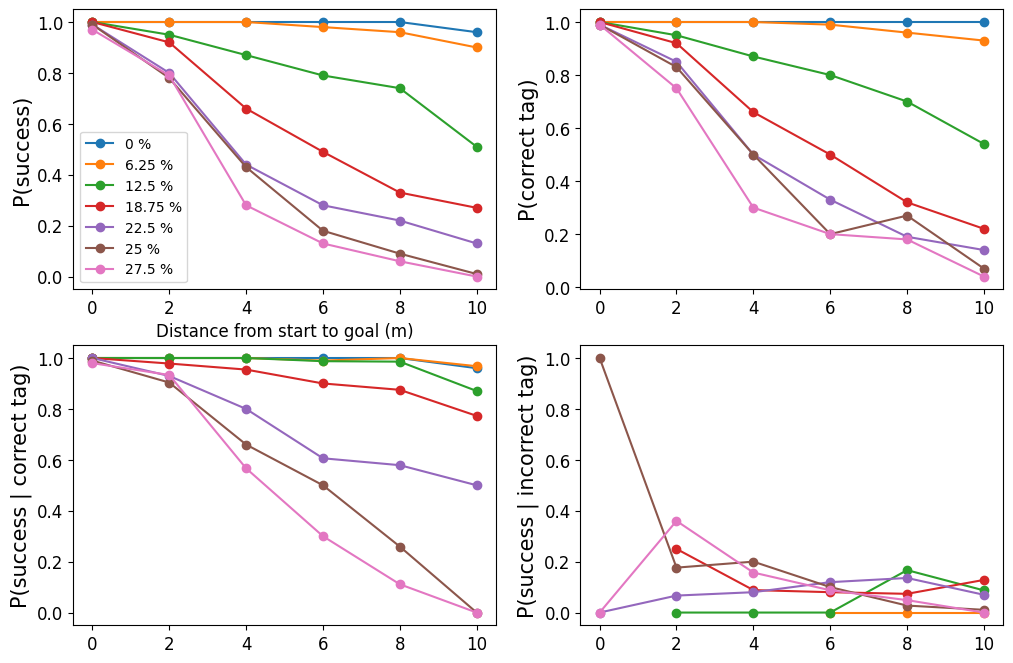
\includegraphics[width=\linewidth]{success_rates_thesis.png}
    \caption{Measures of success and correct tagging as a function of distance from start to goal with different levels of noise. Each point represents the mean across 100 simulations. A simulation was deemed successful if three consecutive iterations were completed in 0.75 times the first iteration, and it was correctly tagged if all tagged cells were reachable via valid transitions across tagged cells from the target cell. Success rates suffer quickly with distance already at 12.5 \% noise, which is reflected in he probability in correctly tagging. Looking only at simulations that only handed out correct tags, success rates were higher, and for higher noise levels. Meanwhile, for almost all simulations, incorrectly tagging indicated low success probability regardless of distance. For the bottom two plots, notice that each point is no longer the mean of 100 - for instance, only a single simulation at 15 \% noise had incorrect tag at 0 distance, which happened to be successful.}
\end{figure}

The success-rate of this model, as a function of distance from start to goal, was heavily dependent on noise in initial delay (figure 2). Although it wasn't quantified, there seemed to be two reasons for the failure of this model, both influenced by this noise level. First, with this learning signal, false positives are still positive. Particularly with high levels of noise, the proportion of false positives is quite high (I think I have data to show this, but I'll need to check. I recall running (or trying to run) an analysis in which I checked if each tagged cell is reachable across valid transitions from all other tagged cells - a geodesic clustering, I guess). With large amounts of noise, the travelling wave is less coherent, with more stray signals. Cells that activate at the right time to get the inhibitory signal might get a stray activation signal and interpret it as a correct feedback signal.

The second reason for failure is that lateral tagged cells in the same layer activate each other, instead of activating a tagged cell in a next layer closer to the target. At low levels of noise, tagged cells in upcoming layers are guaranteed to have a lower delay than tagged cells in the current  layer, because they have received delay-reduction more times. This is not guaranteed with high levels of noise.

Not only will this increase the time from start to target, this signal might never reach the target because it can get stuck in loops between tagged cells in the same layer. When tagged cells activate like this, they will also receive subsequent learning signals, reducing their delay and prevent activation of other cells further.

\subsection{Discussion}
Using activation delay as a learning variable is a fascinating opportunity that arises in continuous-time networks. This has been tried in other networks (I have some sources here, trust me), but those networks typically used Markovian transitions  to simulate single paths, eventually converging on the shortest path but requiring more time. These simulations also used eligibility traces, but these were coupled with more typical reward signals upon reaching the goal, as seen in other papers (more sources here).

As opposed to these networks, this simulation was more reminiscent of Dijkstra's algorithm, simulating all paths in parallel (source here, and it is at least pseudo-correct to say that Dijkstra's works in parallel, right, or should I use another word?). This is more in line with the TSS model, which allows a place cell to transition to all surrounding place cells through a transition network. Importantly for this model, it was only through this transition network that place cells knew who exactly their neighbors were - neither the inhibitory signal nor the learning rules depended on proximity information beyond that given across the transition network.

Another difference between this model and previous models is that it doesn't use an eligibility trace coupled with a reward signal, but two traces. In addition, these traces weren't understood as decaying signals, but rather a signal that increased, followed by a decay.

The motivation for this temporal development of the eligibility trace is that it allowed place cells to avoid getting tagged if the learning signal arrived too soon, because in that case the learning signal couldn't have been evoked by that place cell. This shows that this model tries to solve a problem analogous to the one backpropagation tries to solve, but in a biologically plausible way: when some beneficial cell is activated, such as the target cell, which cells should be rewarded for participating in that activation?
In backpropagation or backpropagation through time, this is solved by remembering all neural activations and interactions across time, so that by the time the target neuron is active, this separate memory can be used to compute the role each cell has. There is little to no evidence that the brain does this, or that a neural network can implement this separate memory structure efficiently. 

Meanwhile, for the previously mentioned delay-learning simulations with Markovian activation dynamics, the reward signal released upon target-activation is sufficient because the relevance of a given place cell is directly dependent on that place cell's activation time, so a single eligibility trace is enough to let the cell know its own role in the activation. In a travelling wave with no direction bias, the activation time is not correlated to path-relevance, making this learning rule obsolete.

A combination of these two was sought in this work. It is at most deemed a partial success, because of its struggle to converge for long distances and higher noise levels. More specifically, the role of inhibition should probably be closely scrutinized for this method to bear fruits. For this particular problem, finding a unique path across a series of connected neurons, inhibition might be merited because it is important to prevent all unwanted place cells from activating.

However, as described in the results, the dynamics here are highly dependent on precise inhibition-timing, so its fragile to noise and can end up in loops. Moreover, the double eligibility trace is missing something to guarantee convergence. In some sense, the inhibitory signal can be seen as a temporal filter, so only cells that are activated at the right time can receive the learning signal. The feedback signal can be understood as a location filter, because it is conveyed via the transition network. Both of these signals come with constraints. The inhibitory signal limits the network activity, because the network must tolerate frequent total inhibition. The feedback signal is limited because it's anonymous as a regular activation signal. This is necessary, because it move across the transition layer, which shouldn't carry information about tags or delays.

These represent problem-areas to focus on before this pathfinding model is deemed highly functional. While this work focused primarily on simulations and testing in an engineer-like fashion, advanced can probably be made with more theoretical and mathematical considerations. Following ideas from TSS, it would also be interesting to implement transitions on multiple scales, for instance by reflexively increasing scale after a given number of transitions.

\end{document}